\chapter{Background} \label{background}

Skylab is built using Ruby on Rails, a well-known web development framework with a great support from a large community, used widely in the industries by companies like Twitter, Groupon, Bloomberg, Airbnb and many more\cite{citation1}. There are many reasons why we have chosen Ruby on Rails. Firstly, Ruby is clean, elegant and easy to read and this feature enables programmers to be more productive. Secondly, Ruby on Rails is adopting many advanced industrial conventions and this enables contributors to have good exposure to programming in the industry. What is more, scaffolding and many gems can significantly boost the productivity. Last but not least, Ruby on Rails community has a favor for open source contribution which aligns well with the open source nature of Skylab.

For the selection of database, we used PostgreSQL. Part of the reason is that it is open source and quite mature, with good drivers available in many languages\cite{citation2}. Besides, we need full ACID compliance for consistency of data and we do not need scalability to multiple servers in the foreseeable future. And PostgreSQL has recently added implementation for rich data structures such as JSON which would make development much easier\cite{citation3}.

Puma is the web server we have chosen for Skylab. Among Passenger, Unicorn, Rainbows! and Puma, Puma is considered to be fast and memory friendly according to online benchmarking\cite{citation4}. Puma is built for high-concurrency and speed and more and more developers to switching to Puma in Rails community\cite{citation5}.

We have selected Nginx as our HTTP server. Nginx has grown in popularity since its release due to its light-weight resource utilization and its ability to scale easily with low memory usage. It excels at serving static content quickly and is designed to pass dynamic requests off to other software that is better suited for those purposes\cite{citation6}. There are also some benchmarking results that indicate the superiority in Nginx handling concurrent access and low memory usage of Nginx\cite{citation7}.

A high-level overview of the architecture of Skylab is illustrated in Figure~\ref{fig:Skylabarch}. Incoming requests to server will first be forwarded to Puma worker processes by Nginx. After that the corresponding Skylab code in Ruby on Rails framework will be executed and when accessing database is required, PostgreSQL will come into picture and serve the data. 

\begin{figure}[h]
  \centering
  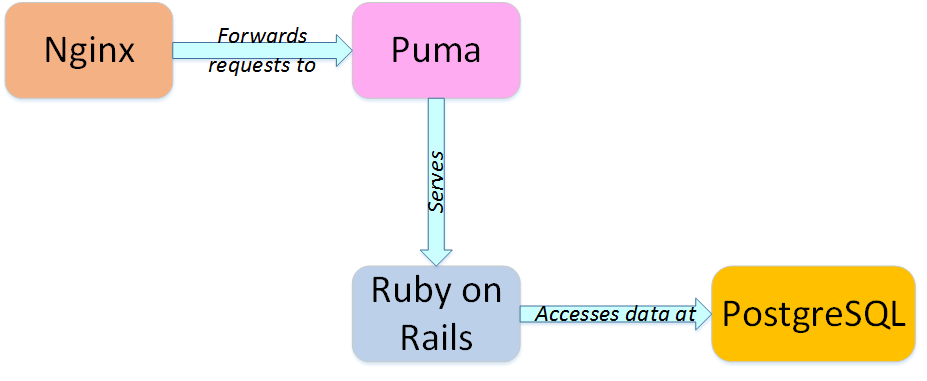
\includegraphics[width=0.85\textwidth]{Images/Skylab_arch.png}
  \caption{Architecture of Skylab}
  \label{fig:Skylabarch}
\end{figure}

\section{System design}

The basic MVC structure of Rails is shown in Figure~\ref{fig:RailsMVC}\cite{citationMVC}:

\begin{figure}[h]
  \centering
  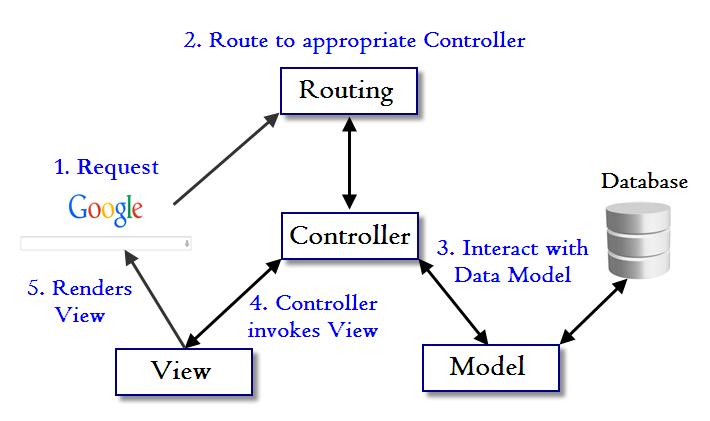
\includegraphics[width=0.85\textwidth]{Images/Rails_MVC.png}
  \caption{Illustration of how MCV works in Rails}
  \label{fig:RailsMVC}
\end{figure}

After request is received by Ruby on Rails framework, the router will look at the pattern of the requested URL path and send it to the corresponding method of the target controller class. The controller is supposed to query models and gather necessary information for rendering the view for user. Last but not least, the response will be sent back to user for viewing.

So the most fundamental component in this whole process is model, which stores all the business data. A good design of model can in fact save a lot of trouble when it comes to writing controller code.

\begin{figure}[h]
  \centering
  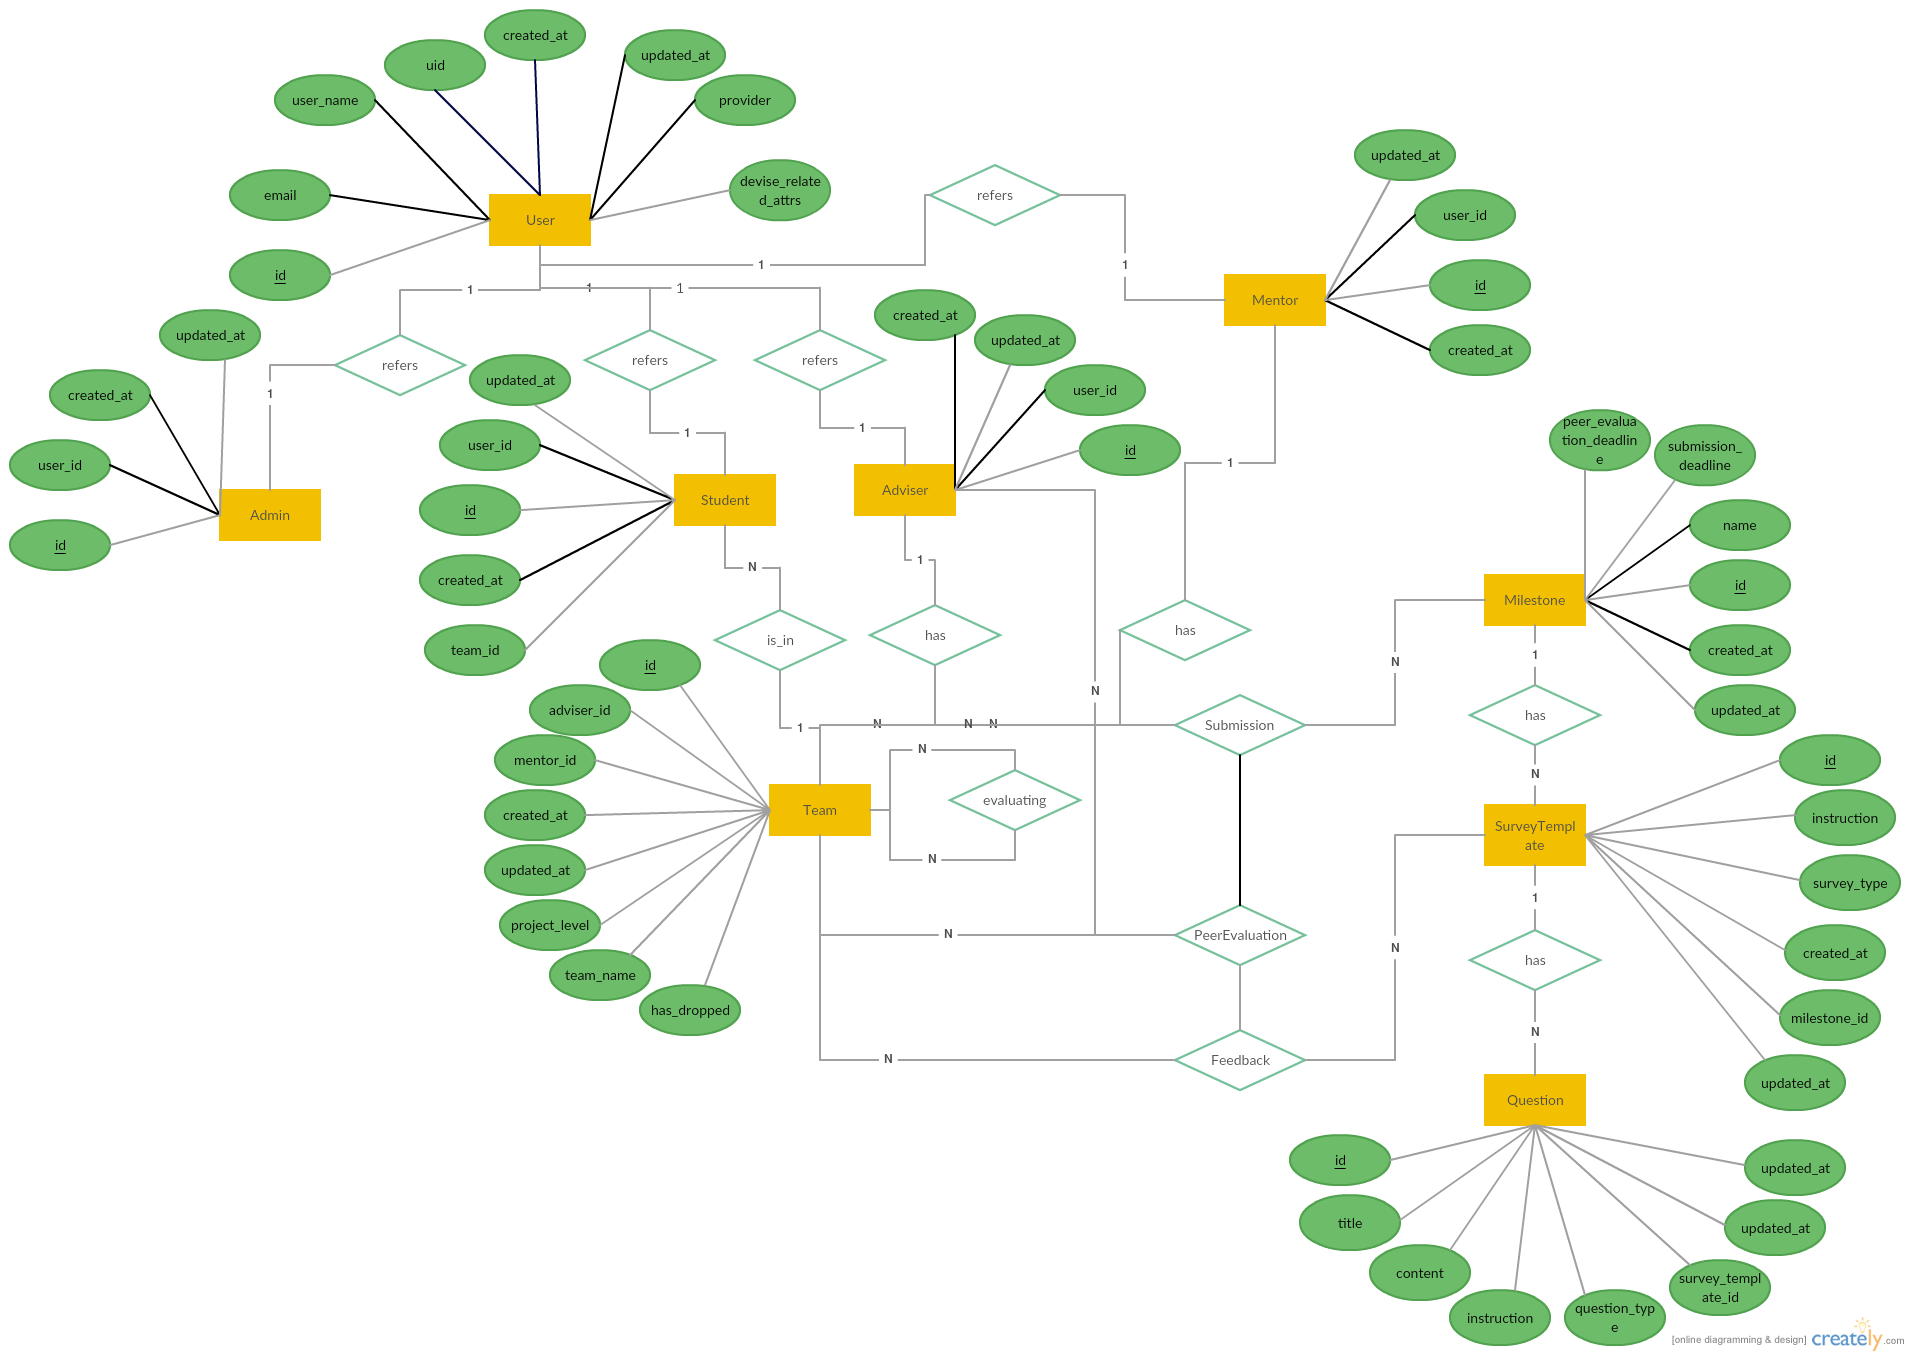
\includegraphics[width=\textwidth]{Images/Skylab_ER.png}
  \caption{Current ER diagram for Skylab}
  \label{fig:SkylabER}
\end{figure}

As you can see from the entity relation diagram shown in Figure~\ref{fig:SkylabER}, users' basic information is captured in the \textit{User} model and each user may have different roles such as \textit{Admin}, \textit{Student}, \textit{Adviser}, \textit{Mentor}. Each student has a \textit{Team} and a team has an \textit{Adviser} and a \textit{Mentor}. Each team will create \textit{Submissions} to \textit{Milestones} to report their progress and assigned evaluator teams will submit \textit{PeerEvaluations} to their \textit{Submissions}. A \textit{SurveyTemplate} contains \textit{Questions} for a \textit{Feedback}, which is for evaluated team to provide feedback to their evaluator teams.

Controllers are crucial in powering a Rails application and in Skylab we have well-defined controllers to carry different tasks. A list of controllers is as follows:

\begin{itemize}
  \item \textbf{AdminsConroller}: handles listing of all Admins, display of an Admin, creation and update of an Admin as well as deletion of an Admin.
  \item \textbf{AdvisersConroller}: handles listing of all Advisers, display of an Adviser, creation and update of an Adviser as well as deletion of an Adviser.
  \item \textbf{EvaluatingsConroller}: handles listing of all evaluation relationships, creation and update of an evaluation relationship as well as deletion of evaluation relationship.
  \item \textbf{FeedbacksConroller}: handles creation and update of a Feedback.
  \item \textbf{HomeConroller}: handles serving of homepage.
  \item \textbf{MentorsConroller}: handles listing of all Mentors, display of a Mentor, creation and update of a Mentor as well as deletion of a Mentor.
  \item \textbf{MilestonesConroller}: handles listing of all Milestones, display of a Milestone, creation and update of a Milestone as well as deletion of a Milestone.
  \item \textbf{PeerEvaluationsConroller}: handles creation and update of a PeerEvaluation.
  \item \textbf{ReceivedEvalsConroller}: handles listing of all received peer evaluations by a team for one milestone.
  \item \textbf{ReceivedFeedbacksConroller}: handles listing of all received feedbacks by a team for one milestone.
  \item \textbf{StudentsConroller}: handles listing of all Students, display of a Student, creation and update of a Student as well as deletion of a Student.
  \item \textbf{SubmissionsConroller}: handles display of a Submission, creation and update of a Submission.
  \item \textbf{SurveyTemplatesConroller}: handles listing of all SurveyTemplates, creation and update of a SurveyTemplate as well as deletion of a SurveyTemplate.
  \item \textbf{TeamsConroller}: handles listing of all Teams, display of a Team, creation and update of a Team as well as deletion of a Team.
  \item \textbf{UsersConroller}: handles listing of all Users, display of a User, creation and update of a User as well as deletion of a User.
  \item \textbf{auth}: handles authentication related to Devise and OpenID.
  \item \textbf{public\_views}: handles serving of publicly available information.
\end{itemize}

\section{Development process}

As Skylab is a web application for which version does not mean anything in particular, we have adopted GitHub flow in our development process\cite{citation8}. So the master branch always contains the latest stable and deployable code base. Each feature will be developed on a feature branch and once the feature is ready, a pull request is created against master. After code review and all tests passes, pull requests will be merged into master and ready for deployment. Figure~\ref{fig:GithubFlow} illustrates the process as well\cite{citation8}.

\begin{figure}[h]
  \centering
  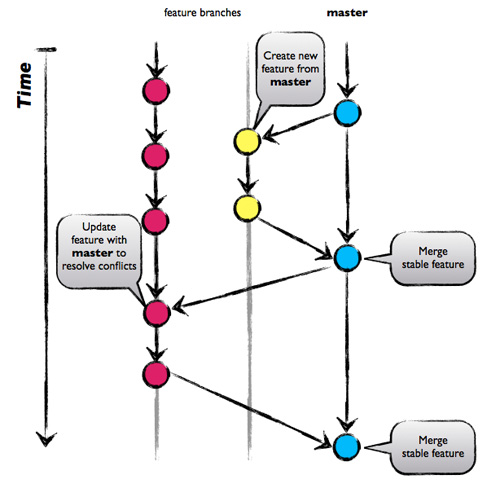
\includegraphics[width=0.7\textwidth]{Images/Github_Flow_Branching_Model.jpg}
  \caption{Branching diagram for GitHub Flow}
  \label{fig:GithubFlow}
\end{figure}

By using GitHub flow and services such as Travis as the continuous integration service, CodeClimate as the code quality monitoring service, we can keep the development of Skylab agile and fast. Besides GitHub flow has enabled Skylab to deployed regularly, which is essential for timely improvement of user experience\cite{citation9}.
